%===============================================================================
% Zentrale Layout-Angaben und Befehle
%===============================================================================
%
% Für bessere Sicht von falschen Umbrüchen die Option draft benutzen.
% Dadurch können aber die eingebundenen Bilder nicht sichtbar sein.
\documentclass[a4paper, 12pt]{article}
%
% Hier zunächst die benötigten Packages
\usepackage[utf8]{inputenc}
\usepackage{fancyhdr}
\usepackage[T1]{fontenc}
\usepackage{ae}
\usepackage{listings}
\usepackage{color}
\usepackage{listings}
\usepackage{wrapfig}
\usepackage[printonlyused]{acronym}
\usepackage{url}
\usepackage{hyperref}
%
% Einbindung des Grafik-Pakets
\ifx\pdfoutput\undefined
	\usepackage[dvips]{graphicx}
\else
	\usepackage[pdftex]{graphicx}
	\pdfcompresslevel=9
	\pdfpageheight=297mm
	\pdfpagewidth=210mm
\fi
%
% Page-Layout
\setlength\headheight{14pt}
\setlength\topmargin{-15,4mm}
\setlength\oddsidemargin{-0,4mm}
\setlength\evensidemargin{-0,4mm}
\setlength\textwidth{160mm}
\setlength\textheight{252mm}
%
% Absatzeinstellungen
\setlength\parindent{0mm}
\setlength\parskip{2ex}
%
% Kopf- und Fusszeile
\pagestyle{fancy}
\fancyhf{} % alles löschen
\fancyhead[LO]{\footnotesize\sc\nouppercase{\leftmark}}
\fancyfoot[LO]{\footnotesize\sc Professur für Angewandte Informatik, insbesondere Smart Environments }
\fancyfoot[RO]{\thepage}
\renewcommand{\headrulewidth}{0pt}
\renewcommand{\footrulewidth}{0pt}
%
% Bessere Fehlermeldungen
\errorcontextlines=999
%
% Anweisung zur Erstellung der Titelseite
% #1 Bachelorarbeit || Masterarbeit
% #2 = Studiengang
% #3 = Titel der Arbeit
% #4 = Autor
% #5 = Abgabedatum
\renewcommand{\maketitle}[5]
{
	\pagenumbering{Alph}
	\begin{titlepage}
		\centering
		\begin{minipage}[t]{16cm}
			\begin{minipage}{3cm}
				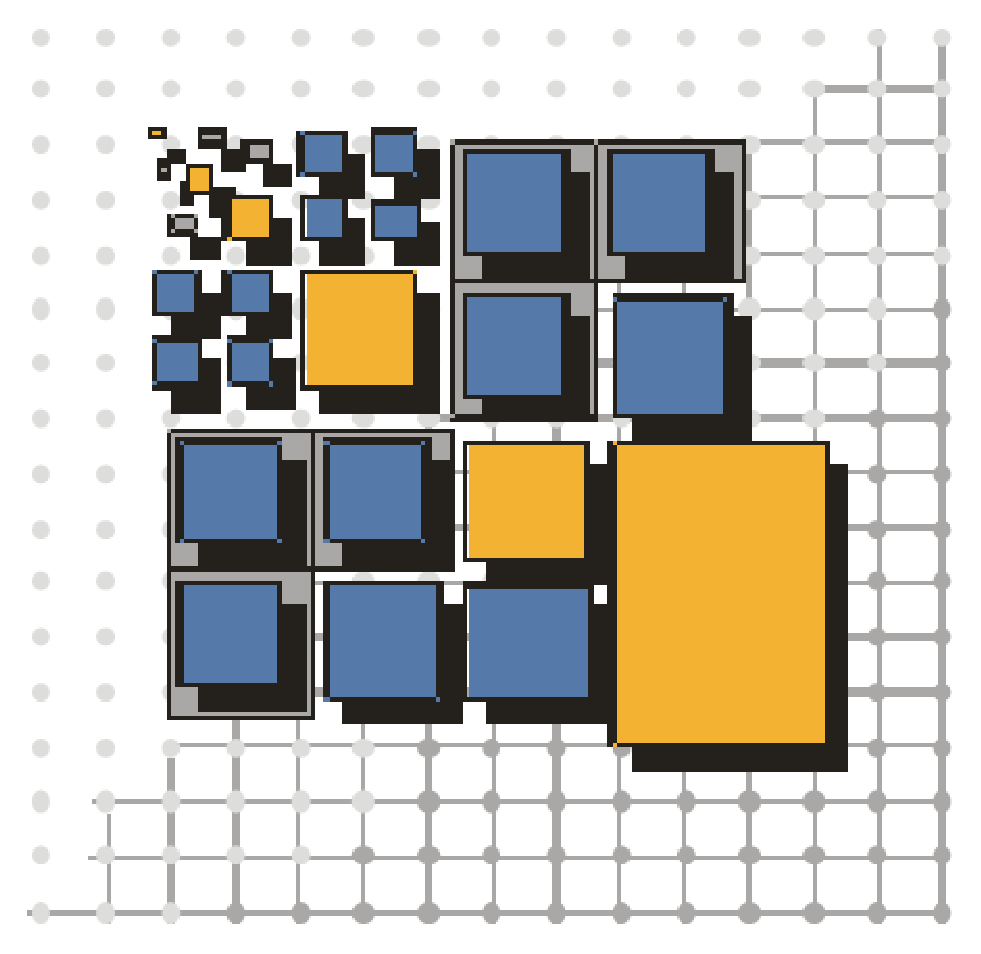
\includegraphics[height=26mm]{includes/vs-logo}
			\end{minipage}
			\hfill
			\begin{minipage}{9cm}
				\centering
				University of Bamberg\\[12pt]
				{\Large Professur für Angewandte Informatik, insbesondere Smart Environments}
			\end{minipage}
			\hfill
			\begin{minipage}{3cm}
				
\includegraphics[height=26mm]{includes/UB-Logo-neu_blau-cmyk}
			\end{minipage}
		\end{minipage}\\[130pt]
		{\LARGE #1}\\[24pt]
		in the degree programme #2\\
		at the Faculty of Information Systems and Applied Computer Sciences,\\ University of Bamberg\\[90pt]
		Topic:\\[24pt]
		{\Huge #3}\\[60pt]
		\vfill
		\begin{minipage}{\textwidth}
			\center
			Author:\\
			{\Large #4\\[12pt]}
			Reviewer:\\
			Prof. Dr. Diedrich Wolter\\[12pt]
			Date of submission:\\
			#5\\
		\end{minipage}
	\end{titlepage}
}
%
% Anweisung zur Erstellung der Eigenständigkeitserklärung
% #1 = Typ der Arbeit
% #2 = Datum
% #3 = Vorname Name
\newcommand{\makedeclaration}[3]
{
	\fancyhead[LO]{\footnotesize\sc\nouppercase{Declaration}}
	%
	\vspace*{16cm}
	In accordance with § 9 Para. 12 APO, I hereby declare that I wrote the preceding #1 independently and did not use any sources or aids other than those indicated. Furthermore, I declare that the digital version corresponds without exception in content and wording to the printed copy of the #1 and that I am aware that this digital version may be subjected to a software-aided, anonymised plagiarism inspection.
	\vspace*{1cm}
	
	Bamberg, #2 \hspace{5cm} #3
	%
}
%
% Wird für Hintergrund von Codelistings benötigt
\definecolor{hellgrau}{gray}{0.9}
%
% Einstellungen für Java-Code
\lstdefinestyle{javaStyle}{%
	basicstyle=\small,%
	backgroundcolor=\color{hellgrau},%
	keywordstyle=\bfseries,%
	showstringspaces=false,%
	numbers=left,%
	numberstyle=\footnotesize,%
	stepnumber=1,%
	numbersep=3pt,%
	extendedchars=true,%
	xleftmargin=2em,%
	lineskip=-1pt,%
	tabsize=4,%
	language=Java,
	breaklines,%
	identifierstyle=\ttfamily,
}
%
% neues environment für Java-Sourcecode
% #1 = "caption={Hier eigene Überschrift}, label={Hier eigenes Label}"
\lstnewenvironment{javacode}[1][]{%
	\lstset{style=javaStyle,#1}%
}{}
%
% Befehl zum Einbinden von Java-Sourcecode aus Datei
% #1 = Dateiname relativ zu src-Verzeichnis
% #2 = Überschrift
% #3 = Label
\newcommand{\javafile}[3]{%
	\lstinputlisting[%
		caption={#2},%
		label={#3},%
		style=javaStyle]{src/#1}%
}
%
% Einbindung eines Bildes
% #1 = label für \ref-Verweise
% #2 = Name des Bildes ohne Endung relativ zu images-Verzeichnis
% #3 = Beschriftung
% #4 = Breite des Bildes im Dokument in cm
\newcommand{\asfigure}[4]{%
	\begin{figure}[htb]%
		\begin{center}%
			\includegraphics[width=#4cm]{images/#2}%
			\vskip -0.3cm%
			\caption{#3}%
			\vskip -0,2cm%
			\label{#1}%
		\end{center}%
	\end{figure}%
}
%
% Umgebung für Fliesstext um Grafik
% #1 = Ausrichtung: r, l, i, ...
% #2 = Breite des Bildes in cm
% #3 = Name des Bildes ohne Endung relativ zu images-Verzeichnis
% #4 = Beschriftung
% #5 = label für \ref-Verweise
\newcommand{\textflow}[5]{%
	\begin{wrapfigure}{#1}{#2cm}%
		\includegraphics[width=#2cm]{images/#3}%
		\caption{#4}%
		\label{#5}%
	\end{wrapfigure}%
}
%%% Local Variables:
%%% mode: latex
%%% TeX-master: t
%%% End:
